\chapter{Image Data Collection using Autonomous Drone}

\section{About}

This chapter deals with complete specifications of our vehicle used for the penultimate applications of using for precision farming applications. The focus of this chapter is to lay out a complete overview of our system used with the causes and outputs related to the precision farming applications. Which flight mode is to be used at what time, how would those flight modes be accessed, significance of PID Autotune, why making a dataset of farm images is necessary, etc. are some of the questions we have tried to answer in this chapter. 

During our field tests, the drone was powered by a 2200 mAh (milliampere-hour) battery, which allowed it to fly for around 25 minutes per mission, and over a total distance of approximately 15 km. Using the APM Planner (version 1.1.26), we programmed the flight path of each mission by clicking on waypoints in a Google satellite map interface. The drone can be programmed to take off and land autonomously, and circle over any waypoint for a specified number of turns or duration. We also programmed other flight parameters such as ground speed and altitude of each waypoint. Each pre-programmed mission was uploaded to the drone, which would then fly the mission autonomously.


We would be discussing the overview, selection of flight controller, detailed specification of physical parameters used by our system, sensors used for our application, flight modes representing Autotune, Loiter mode(hover) and guided waypoint ultimately resulting in an autonomous flight. We would be making the dataset of images available as open-source so that public can utilize this data for machine learning purposes. 

The overall pipeline showcasing the system flow is displayed in Fig.~\ref{fig: asda}

\begin{figure}[!h]
	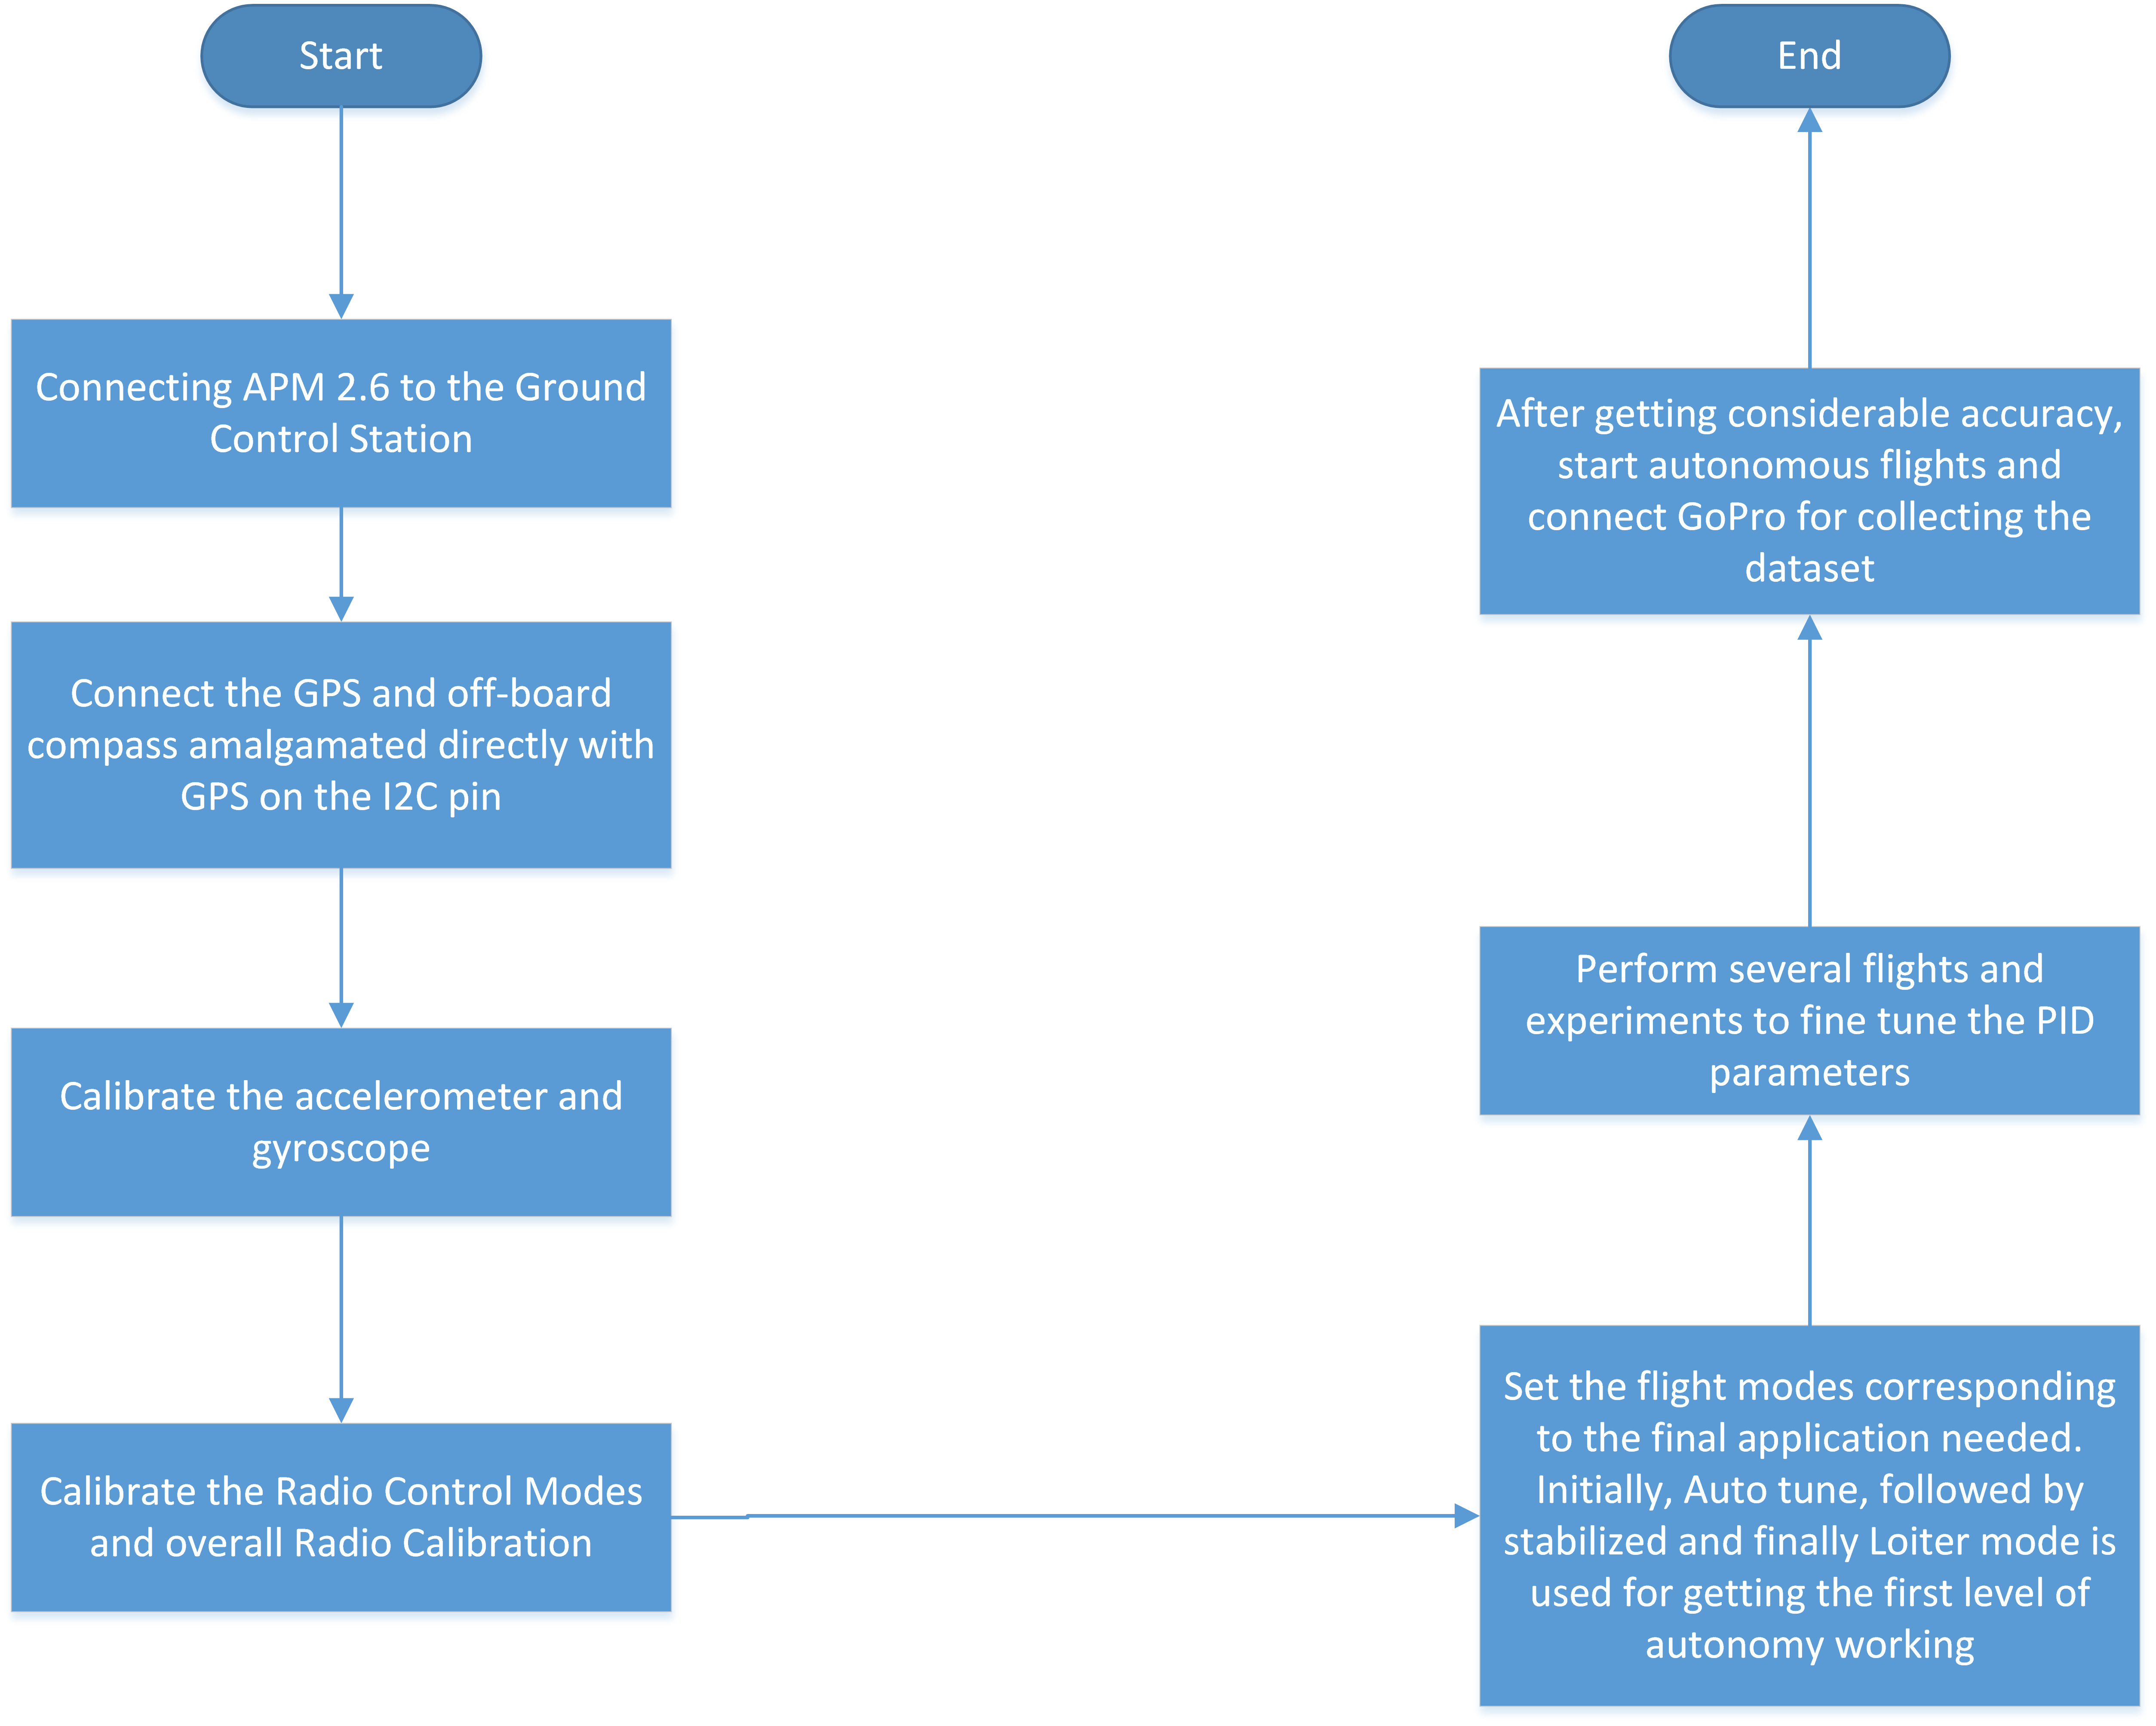
\includegraphics[width=1.0\linewidth]{asda}
	\centering
	\caption{\label{fig: asda}Pipeline of the autonomous hex-copter flight system}
\end{figure}.
A proper working sytem of the pipeline shown in Fig.~\ref{fig: asda} is accomplished and displayed in chapter ``Chapter 7 - Experimental Results''.


\section{Overview of the System}


The reason we zeroed in on using the overview flow as shown in Fig.~\ref{fig: img_1} and using APM system was because it is an open-source autopilot solution for multi-rotor vehicles, offering both enhanced remote control flight (via a number of intelligent flight modes) and execution of fully autonomous missions~\cite{19}. As part of the wider ArduPilot software platform it works seamlessly with Ground Control Station software that can monitor vehicle telemetry and perform powerful mission planning activities. It also benefits from other parts of the Ardupilot ecosystem, including simulators, log analysis tools, and higher level APIs for vehicle management and control. 

\begin{figure}[h]
	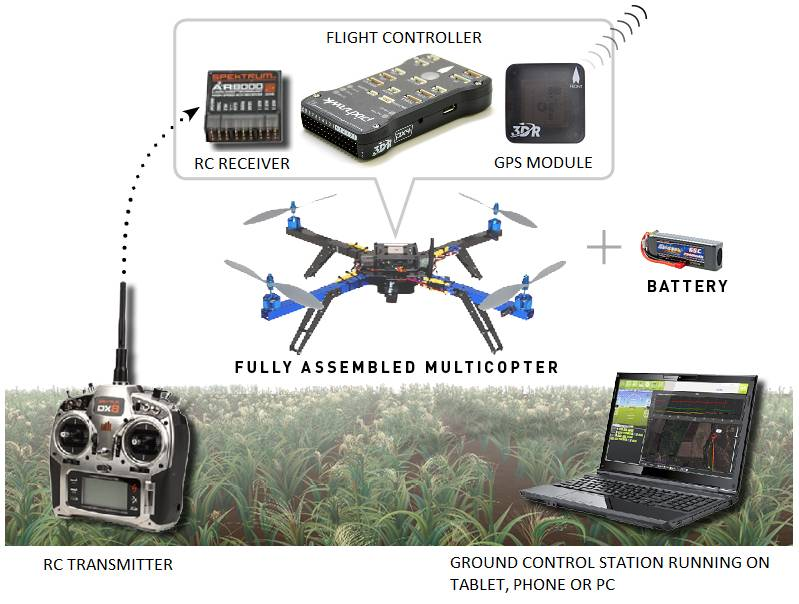
\includegraphics[width=0.9\linewidth]{img_1}
	\centering
	\caption{\label{fig: img_1}Overview of our system}
\end{figure}.

\subsection{Choosing a Flight Controller}
ArduPilot runs on many different flight controller boards. Selecting the right board depended on the physical restraints of the vehicle and the applications we wanted to run. Due to it's gracious presence and impression in open-source domain and the popularity in its forums, we retained our system to APM 2.6 Flight controller as our need for gathering data by flying upon agricultural fields either with autonomy or hand-held control was being accomplished by this system.


That being the prime reason for choosing APM 2.6 Controller as shown in Fig.~\ref{fig: 3 and 4}. Also, the APM 2.6 board requires no assembly, and is ready for firmware. We have a choice of side or top entry pin configuration, in order to accommodate a variety of installations. 

APM 2.6 is a revision of the APM that makes use of an external compass. Our APM 2.6 had no on board compass, and it is optimized for vehicles where the compass should be placed as far from power and motor sources as possible to avoid magnetic interference. Our APM 2.6 is designed to be used with the 3DR GPS uBlox LEA-6 with Compass module. We mounted the GPS/Compass module further from noise sources than the APM itself. APM 2.6 required a GPS unit with an on board compass for full autonomy, the condition fulfilled by our system.

\begin{figure}[t]
	\hfill
	\subfigure[]{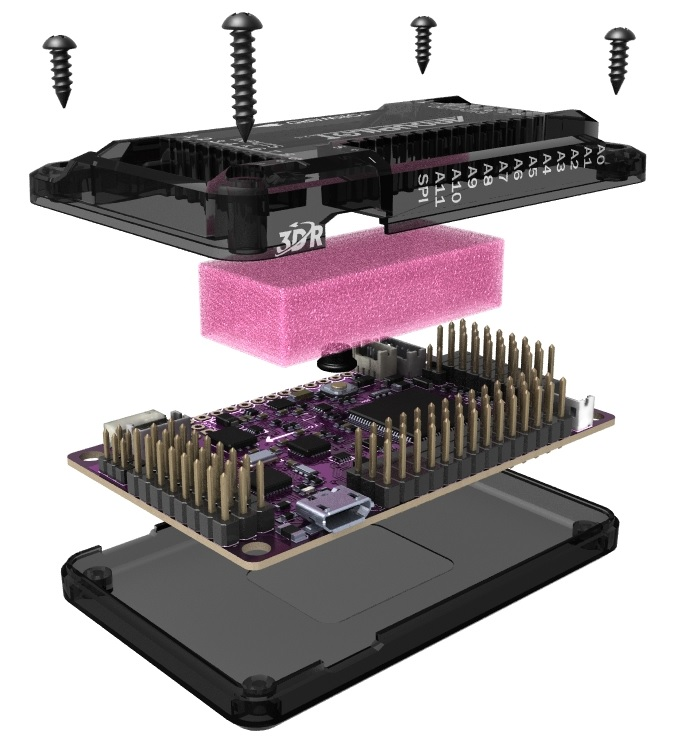
\includegraphics[width=0.48\linewidth]{3}}
	\hfill
	\subfigure[]{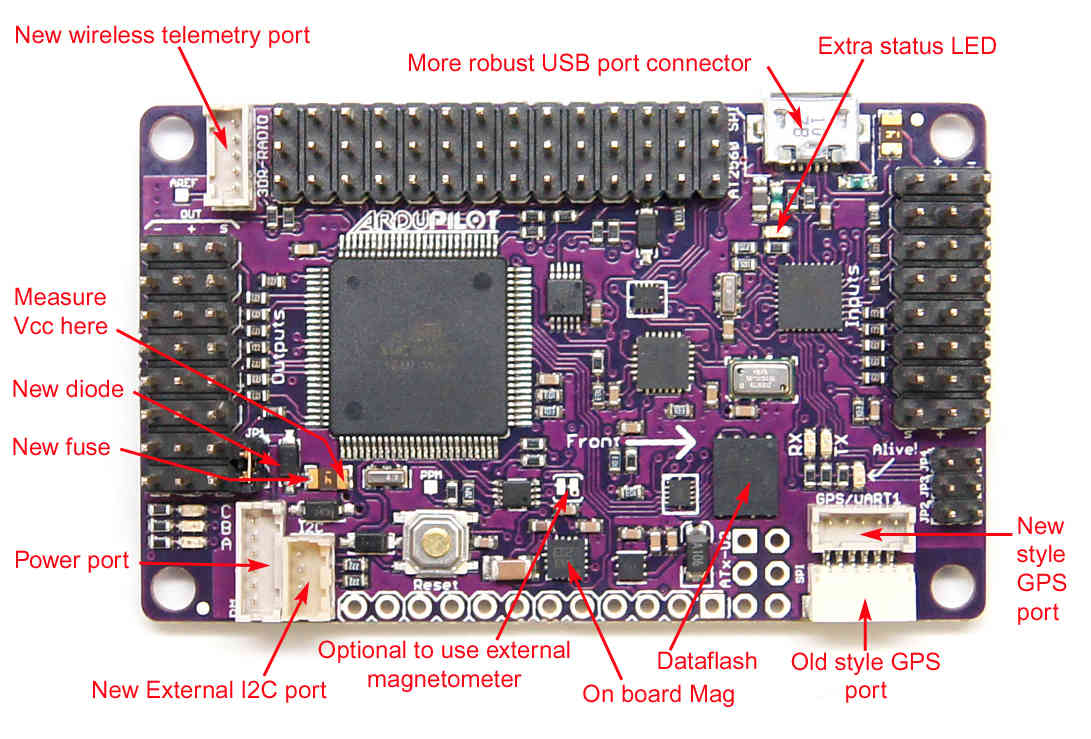
\includegraphics[width=0.48\linewidth]{4}}
	\hfill
	\caption{\label{fig: 3 and 4}APM 2.x overview~\cite{19}}
\end{figure}


\section{Physical Parameters pertaining to our system}
6 brushless DC motors of 1000kV are used on our hex-copter. Detailed specifications of Sensors, Electrical parameters and Mechanical parameters are described below.
\subsection{Sensors}
\begin{itemize}
	\item \textbf{MPU6000}: 3 accelerometers, 3 gyroscopes and 1 temperature sensor
	\item \textbf{MPU9250}: 3 accelerometers , 3 magnetometers, 3 gyroscopes and 1 temperature sensor
	\item \textbf{LSM9DS0}: 3 accelerometers , 3 magnetometers, 3 gyroscopes and 1 temperature sensor
	\item \textbf{MS5611-01BA}: 1 digital pressure sensor (barometer) and 1 temperature sensor
\end{itemize}

\subsection{Electrical}

\begin{itemize}
	\item \textbf{Power}:A 5V Supply, power module connector (DF-13 6 pins), ESC signal cables
	\item \textbf{Indicators}: 3 normal LEDs (Green, Amber and Blue), RGB LED
	\item \textbf{Connectors}: 2x UARTs, 1x ADC connector, 1x CAN, 3x I2C, 1x Buzzer out, 1x Safety switch, 12x PWM output channels, 1 PPM/S.Bus in, 1x Power brick and 1x Battery backup (1 LiPo cell)
\end{itemize}

\subsection{Mechanical}
\begin{itemize}
	\item \textbf{Size}: 95.6 x 75.27 x 36.2 mm
	\item \textbf{Layers}: 6 PCB thickness 1.6 mm
	\item \textbf{RoHS Complicant}: Yes
	\item \textbf{Weight}: 110 grams
\end{itemize}



\section{Remote Control Modes}
\subsection{Overview}
We used RC transmitters that are used to control vehicle movement and orientation. Copter minimally control throttle, pitch, roll and yaw. We mapped each of these control signals to transmitter stick/switch(s) and in turn to autopilot channels from the connected receiver.

We needed to calibrate each of the transmitter controls/channels. For that, simply moved each of the enabled sticks/switches through their full range and record the maximum and minimum positions.

\subsection{Transmitter configuration}
There are two main transmitter configurations on our hex-copter:
\begin{itemize}
	\item \textit{Mode 1}: left stick controls pitch and yaw, the right stick will control throttle and roll. It is shown in Fig.~\ref{fig: mos_1}.
	\item \textit{Mode 2}: left stick controls throttle and yaw; the right stick will control pitch and roll. It is shown in Fig.~\ref{fig: mos_2}.
\end{itemize}
\begin{figure}[h]
	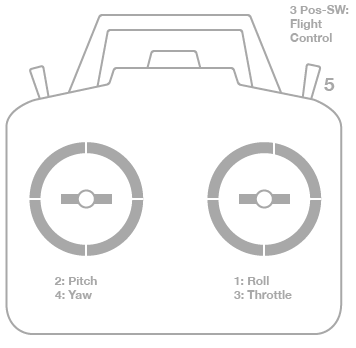
\includegraphics[width=0.5\linewidth]{radio_setup_mode_1}
	\centering
	\caption{\label{fig: mos_1}\textit{Transmitter(Mode 1): Recommended Channels}}
\end{figure}

\begin{figure}[h]
	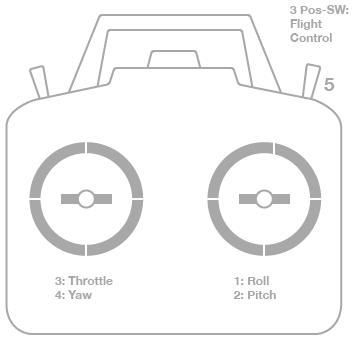
\includegraphics[width=0.5\linewidth]{rc_transmitter_mode2_setup}
	\centering
	\caption{\label{fig: mos_2}\textit{Transmitter(Mode 2): Recommended Channels}}
\end{figure}


\subsection{Channel Mappings}
Copter default channel mappings are:
\begin{itemize}
	\item \textbf{Channel 1}: Roll
	\item \textbf{Channel 2}: Pitch
	\item \textbf{Channel 3}: Throttle
	\item \textbf{Channel 4}: Yaw
	\item \textbf{Channel 5}: Flight Modes
	\item \textbf{Channel 6}: (Optional) Inflight tuning or camera mount (mapped to transmitter tuning knob)
\end{itemize}
Unused channels can be mapped to control additional peripherals.

\subsection{Connecting autopilot and turning on receiver}
We first connected the autopilot via USB and turned on your RC transmitter. Then, we verified that the transmitter is bound to the receiver (the receiver displayed a solid green light) and that it is set to use the correct model for our vehicle.

We then opened Mission Planner’s INITIAL SETUP | Mandatory Hardware | Radio Calibration screen. Since our RC receiver (Rx) and transmitter (Tx) are bound, we saw the green bars move when we moved the transmitter sticks.

\begin{figure}[h]
	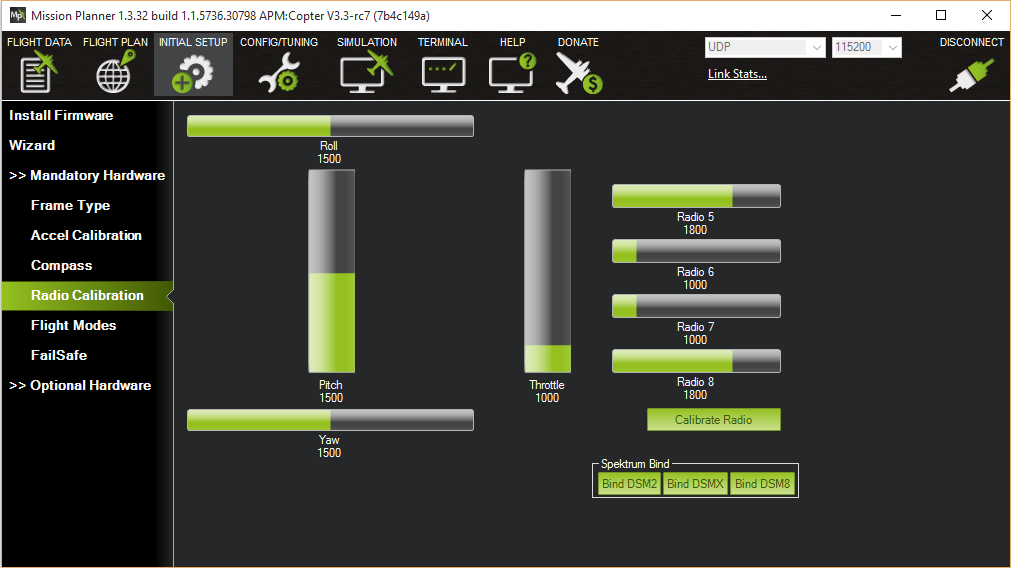
\includegraphics[width=1.0\linewidth]{mp_radio_calibration}
	\centering
	\caption{\label{fig: mos_3}\textit{MissionPlanner: Radio Calibration Screen (Copter)}}
\end{figure}

\subsection{Calibration steps}
\begin{enumerate}
	\item Opened Mission Planner’s INITIAL SETUP | Mandatory Hardware | Radio Calibration screen. A screen shown in Fig.~\ref{fig: mos_3} will be opened.
	\item Clicked on the green Calibrate Radio button in the lower right of the window.
Mission Planner displayed a prompt to check radio control equipment is on, battery is not connected, and propellers are not attached. We then selected OK. Screen shown in Fig.~\ref{fig: mos_4} will appear.
\begin{figure}[h]
	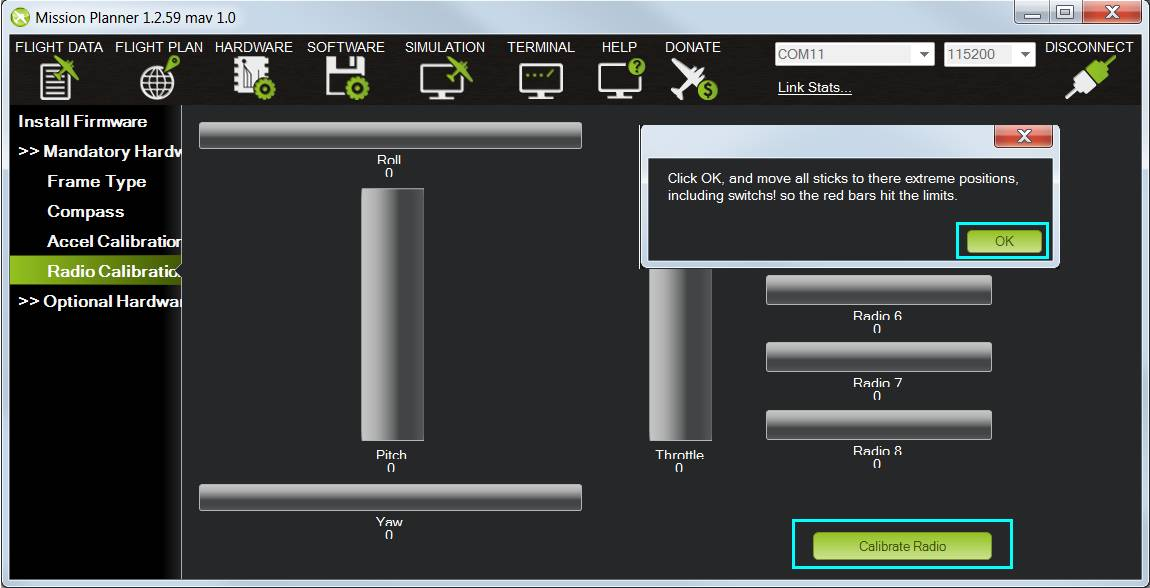
\includegraphics[width=1.0\linewidth]{mp_calibrate_radio}
	\centering
	\caption{\label{fig: mos_4}\textit{Mission Planner: Selected Calibrate Radio and then clicked OK to begin our calibration.}}
\end{figure}
	\item We then moved the control sticks and toggled switches on our transmitter to their limits of travel and observed the results on the radio calibration bars. Red lines appeared across the calibration bars to indicate maximum and minimum values:

\begin{figure}[h]
	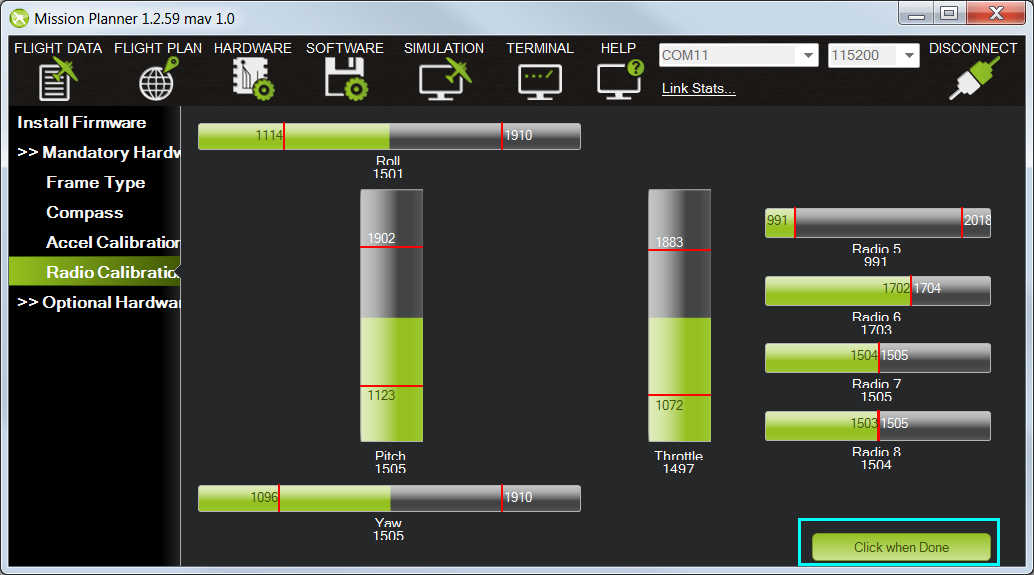
\includegraphics[width=1.0\linewidth]{mp_radio_calibration_click_when_done}
	\centering
	\caption{\label{fig: mos_5}\textit{Mission Planner: Input range marked with red lines}}
\end{figure}
\item Finally, we selected Click when Done when all required channels were set at the minimum and maximum positions.

Mission Planner showed a summary of the calibration data. Normal values are around 1100 for minimums and 1900 for maximums as shown in Fig.~\ref{fig: mos_5}.
\begin{figure}[h]
	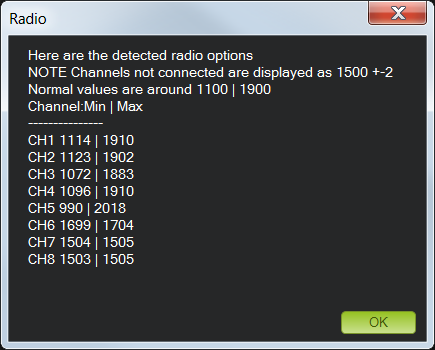
\includegraphics[width=0.7\linewidth]{radi-calib-results}
	\centering
	\caption{\label{fig: mos_6}\textit{Mission Planner: Radio Calibration Results}}
\end{figure}
\item Finally, we turned off our transmitter and disconnect the battery if it was connected and Radio Calibration results as shown in Fig.~\ref{fig: mos_6} appears.

\end{enumerate}

\subsection{RC Transmitter Flight Mode Configuration}
\subsubsection{Flight modes configuration}
The mapping between switch position and flight mode is set in the Mission Planner Flight Mode screen, as shown in Fig.~\ref{fig: mos_7}.

\begin{figure}[h]
	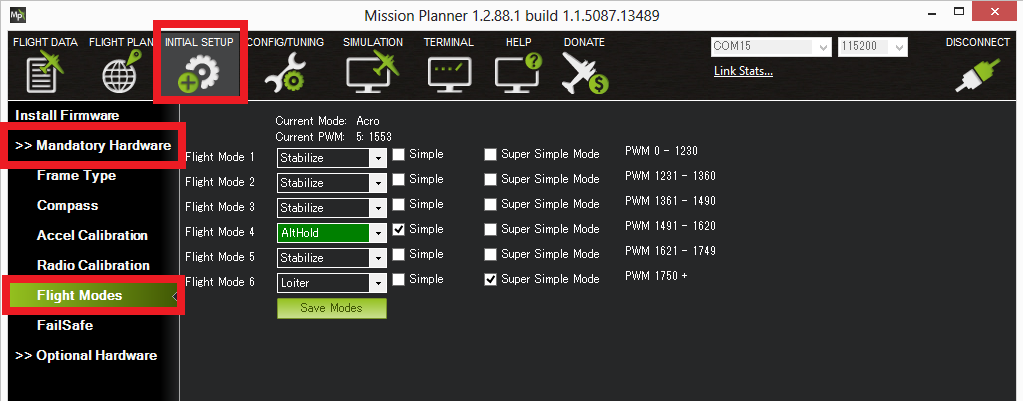
\includegraphics[width=1.0\linewidth]{mp_setup_flight_mode}
	\centering
	\caption{\label{fig: mos_7}\textit{Mission Planner:Flight Mode Screen}}
	\end{figure}
We set up the flight modes available on the transmitter by doing the following:
\begin{itemize}
	\item Turned on our RC transmitter
    \item Connected the APM 2.6 to the Mission Planner
	\item Went to the Initial Setup | Mandatory Hardware | Flight Modes screen
	\item Used the drop-down on each line to select the flight mode for that switch position.
	\item Ensured that at least one switch position is left assigned to STABILISE.
	\item Optionally checked the Simple Mode check-box for that switch position. 
	\item When finished, we pressed the Save Modes button.
	
	Some modes can also be invoked from the auxiliary switches (a.k.a. ch7, ch8 option switches). For example, to set a dedicated switch for RTL.
	
	
\end{itemize}

\subsubsection{Setting the flight mode channel}
The flight mode channel is the input radio channel that ArduPilot monitors for mode changes.
For our case, on our Copter this is always channel 5.

\subsubsection{Transmitter configuration}
The transmitter must emit PWM signals in the correct range to allow us to map a mode to a switch position.
If we wanted to just support three modes (using a three position switch) then we would configure the transmitter to produce PWM pulse widths of 1165, 1425, and 1815 microseconds for the respective switch positions.

If we want to support 6 modes then the transmitter will need to emit PWM widths of around 1165, 1295, 1425, 1555, 1685, and 1815 milliseconds. Typically this is achieved by configuring the transmitter to mix a two position switch and a three position switch (giving 6 modes in total). We can also do this with an analog dial if one is available, but it’s hard to reliably turn a dial to just the right position for six distinct settings.

The sections below provide links showing how to configure transmitters from different manufactures, and how to test (in Mission Planner) that each switch setting is emitting the appropriate PWM signal.

\subsubsection{Test transmitter switch settings}
We can use the Mission Planner Radio Calibration screen to test the PWM pulse widths for each mode setting.

We simply can toggle through the modes on our transmitter and confirm that the PWM for the selected channel matches the required PWM values. The screenshot in Fig.~\ref{fig: mos_8} assumes that the flight mode channel is set to Radio 5.



\begin{figure}[h]
	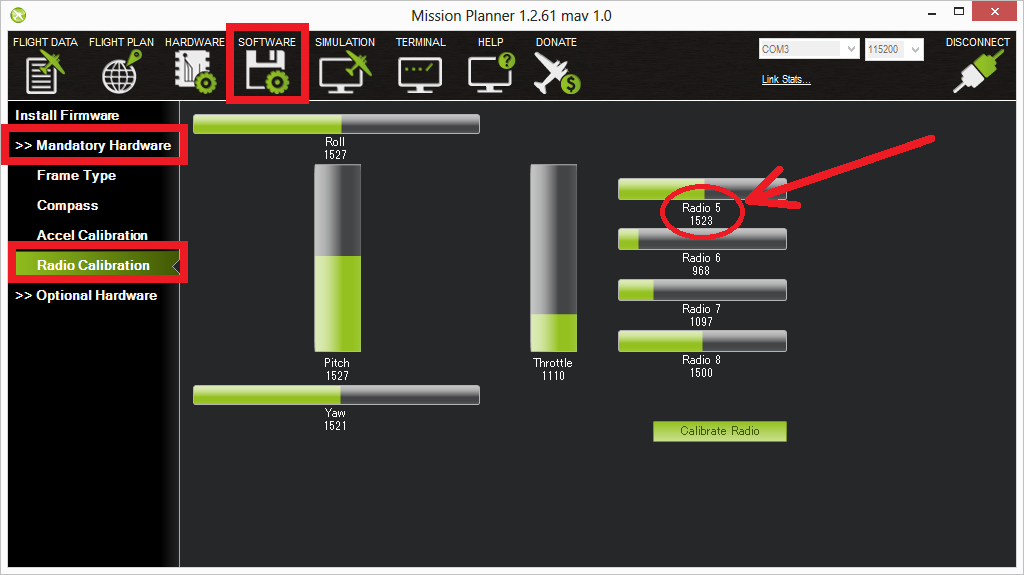
\includegraphics[width=1.0\linewidth]{mp_radio_calibration_ch5_pwm}
	\centering
	\caption{\label{fig: mos_8}\textit{Transmitter switch settings}}
\end{figure}


\section{Flight Modes and Autonomous Navigated Flight}
This section deals with the questions such as why did we end up with following flight modes and how did we went on about doing it.
\begin{itemize}
	\item Autotune Mode
	\item Stabilize Mode
	\item Loiter Mode
	\item RTL Mode
	\item Auto Mode (Autonomous flight)
\end{itemize}

\subsection{Autotune}

In order to get closer to our final aim of an autonomous flight, we needed a stabilized flight. For this, the PID values needed to be calibrated accordingly. Thus, we used this mode to autotune the paramters for a stable flight down the lane while using guided waypoints/auto mode, as shown in Fig.~\ref{fig: AutoTuneCh7Switch}.

AutoTune attempts to automatically tune the Stabilize P, Rate P and D, and maximum rotational accelerations to provide the highest response without significant overshoot. Copter needs to be “basically” flyable in Stabilize mode before attempting to use AutoTune as the feature needs to be able to “twitch” the copter in the roll and pitch axis.
\begin{figure}[h]
	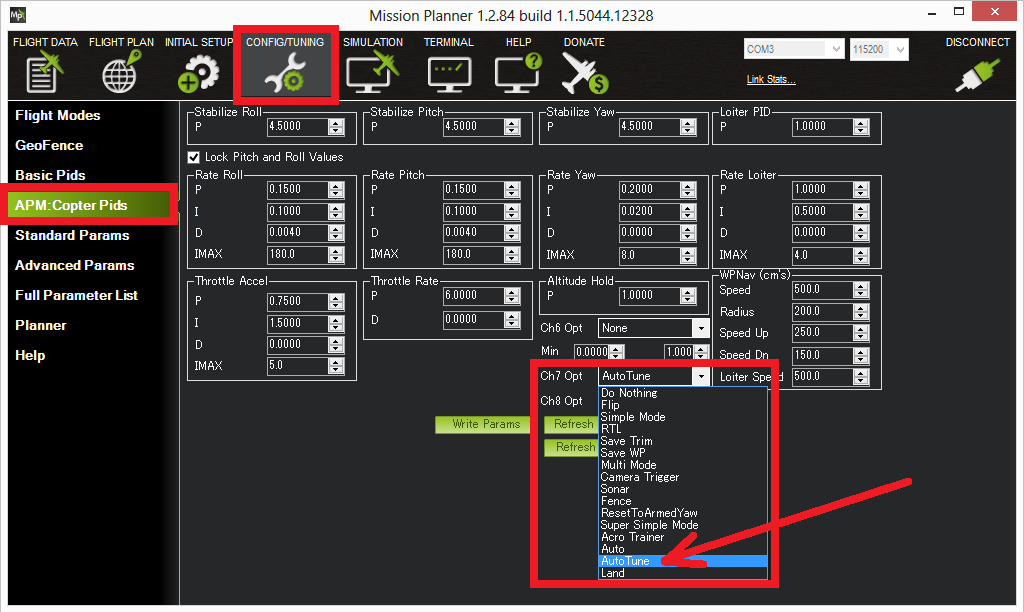
\includegraphics[width=1.0\linewidth]{AutoTuneCh7Switch}
	\centering
	\caption{\label{fig: AutoTuneCh7Switch}\textit{Setup for Autotune}}
\end{figure}

\subsubsection{Setup before flying}
\begin{enumerate}
	\item We set up one flight mode switch position to be AltHold/Stabilize.
	\item Then, we set an Auxiliary Function Switch to Autotune to allow us to turn the auto tuning on/off with the a switch.
\end{enumerate}
\subsubsection{How to invoke AutoTune}
\begin{enumerate}
	\item We waited for a calm day and went to a large open area.
	\item We then ensured that the ch7 or ch8 switch is in the LOW position.
	\item Took off and kept the copter into AltHold/Stabilize mode at a comfortable altitude.
	\item Faced the vehicle so that it will twitch at 90degrees from the direction the wind is blowing (i.e. if tuning Roll first, point the vehicle into the wind). Situation is explained graphically in Fig.~\ref{fig: autotune_copterwind}.
\begin{figure}[h]
	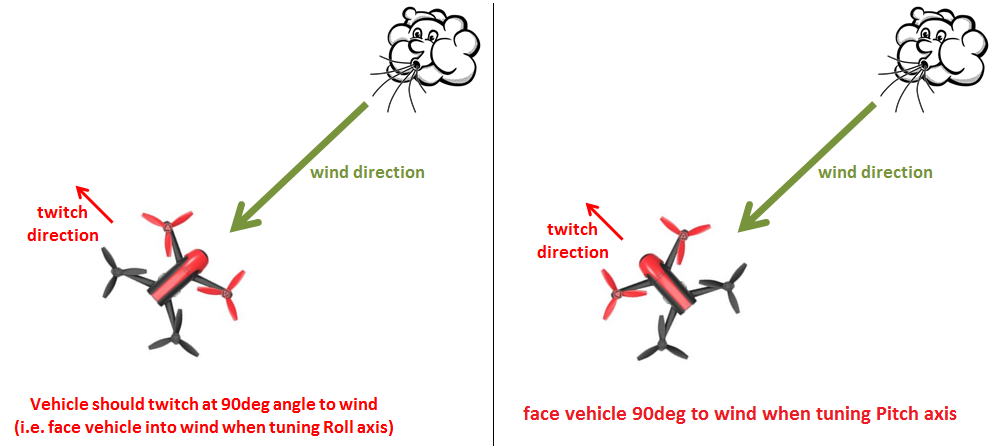
\includegraphics[width=1.0\linewidth]{autotune_copterwind}
	\centering
	\caption{\label{fig: autotune_copterwind}\textit{Twitch direction}}
\end{figure}
	\item Set the ch7/ch8 switch to the HIGH position to engage auto tuning:
	\begin{itemize}
		\item We will see it twitch about 20 degrees left and right for a few minutes, then it will repeat forward and back.
		\item We can use the roll and pitch stick at any time to reposition the copter if it drifts away (it will use the original PID gains during repositioning and between tests). When we release the sticks it will continue auto tuning where it left off.
		\item We can move the ch7/ch8 switch into the LOW position at any time to abandon the autotuning and return to the origin PIDs.
	\end{itemize}
	\item When the tune completes the copter will change back to the original PID gains.
	\item We can put the ch7/ch8 switch into the LOW position then back to the HIGH position to test the tuned PID gains.
	\item Feeling staisfied with the autotuned PID gains, left the ch7/ch8 switch in the HIGH position, landed and disarmed to save the PIDs permanently.
\end{enumerate}
We sometimes found that, after performing an AutoTune, that the vehicle feels overly twitchy when flying Stabilize, AltHold or PosHold (but ok in more autonomous modes like Loiter, RTL, Auto). For this, we tried reducing the RC\_FEEL parameter to $0.25$. This smooths out the given input.

\subsection{Stabilize Mode}
We focused on this mode for our application as this mode allows us to fly our vehicle manually, but self-levels the roll and pitch axis.

\subsubsection{Overview of this mode}
\begin{itemize}
	\item Pilot’s roll and pitch input control the lean angle of the copter. When we release the roll and pitch sticks the vehicle automatically levels itself.
	\item We would need to regularly input roll and pitch commands to keep the vehicle in place as it is pushed around by the wind.
	\item Our yaw input controls the rate of change of the heading. When we release the yaw stick the vehicle will maintain it’s current heading.
	\item Our throttle input controls the average motor speed meaning that constant adjustment of the throttle is required to maintain altitude. If the we put the throttle completely down the motors will go to their minimum rate (MOT\_SPIN\_ARMED) and if the vehicle is flying it will lose attitude control and tumble.
	\item The throttle sent to the motors is automatically adjusted based on the tilt angle of the vehicle (i.e. increased as the vehicle tilts over more) to reduce the compensation we must do as the vehicle’s attitude changes.
	
\end{itemize}
\subsubsection{Tuning}
 We used AutoTune which allowed us to automatically determine the best Stabilize and Rate PID values. 
 
Using this mode, after using the Autotune mode gave us an immense increase in the stability of the flight.



\subsection{Loiter Mode}
This mode was inculcated in our study to verify the first level of autonomy in our flight. This mode enabled us to verify the performance actually carried out by our system when shifted in autonomous mode. By verifying the working of this mode, it was safe for us to assume that we could shift over complete autonomy in guided waypoints mode where our copter flew to corresponding waypoints to achieve an autonomus flight.

Loiter Mode automatically attempts to maintain the current location, heading and altitude. A good GPS lock, low magnetic interference on the compass and low vibrations are all important in achieving good loiter performance.
\subsubsection{Controls}
We can control the copter’s position with the control sticks.

Horizontal location can be adjusted with the the Roll and Pitch control sticks with the default maximum horizontal speed being 5m/s (see Tuning section below on how to adjust this). When we release the sticks the copter will slow to a stop.
Altitude can be controlled with the Throttle control stick just as in AltHold/Stabilize mode
The heading can be set with the Yaw control stick
The vehicle can be armed in Loiter mode but only once the GPS has 3D lock and the HDOP has dropped below 2.0. 


\subsection{RTL Mode}
RTL mode (Return To Launch mode) was needed in our flight to navigate Copter from its current position to hover above the home position. So before/after completing the guided waypoint mission, we could direct our copter to RTL mode so that it may return and hover over the home location before ultimately landing. This mode basically gave control and stabilized our autonomous flight.
\subsubsection{Overview}
When RTL mode is selected, the copter will return to the home location. The copter will first rise to RTL\_ALT before returning home or maintain the current altitude if the current altitude is higher than RTL\_ALT. The default value for RTL\_ALT is 15m. We set it to 5m.

\begin{figure}[h]
	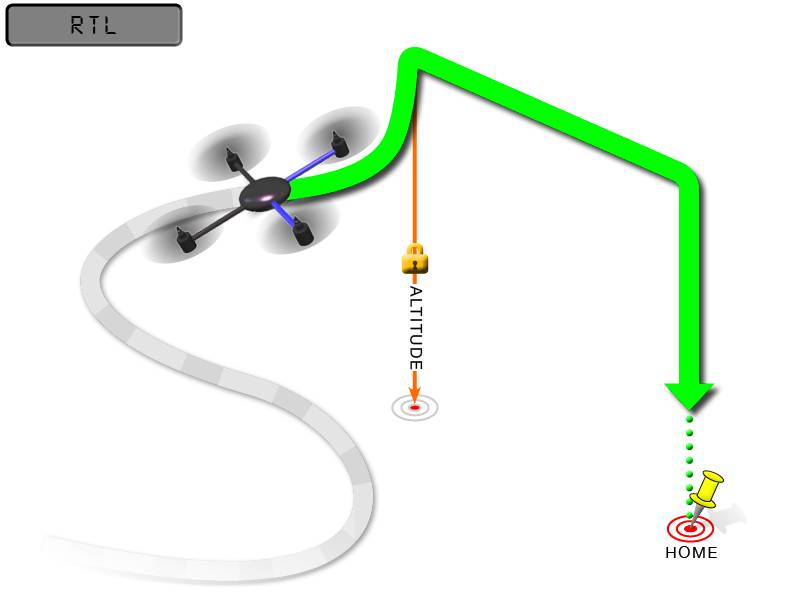
\includegraphics[width=0.7\linewidth]{RTL}
	\centering
	\caption{\label{fig: RTL}\textit{Return to Launch scenario}}
\end{figure}

RTL is a GPS-dependent move, so it was essential that GPS lock was acquired before attempting to use this mode. Before arming, we ensured that the APM’s blue LED is solid and not blinking (for confirmation of GPS fix). For a GPS without compass, the LED will be solid blue when GPS lock is acquired. For the GPS+Compass module, the LED will be blinking blue when GPS is locked(for our case). Figure ~\ref{fig: RTL} aptly describes the RTL Mode execution by our drone.

RTL commanded the copter to return to the home position, meaning that it will return to the location where it was armed. Therefore, the home position is always supposed to be our copter’s actual GPS takeoff location, unobstructed and away from people. For Copter if we get GPS lock and then ARM our copter, the home position is the location the copter was in when it was armed. This means if we execute an RTL in Copter, it will return to the location where it was armed. This is a needed mode while setting up the guided waypoints/Auto method.

\subsection{Auto Mode}
This is the actual mode which we were concerned for since beginning. This gave us the autonomy needed to inspect our crops efficiently and take images(data) by flying over them in a predefined path and taking videos/images using GoPro through a gimbal attached to our hex-copter. All the flight modes explained above were like a prerequisites needed to achive the success in this mode. 

In Auto mode the copter will follow a pre-programmed mission script stored in the autopilot which is made up of navigation commands (i.e. waypoints) and “do” commands (i.e. commands that do not affect the location of the copter including triggering a camera shutter). 
\subsubsection{Overview}
\begin{figure}[h]
	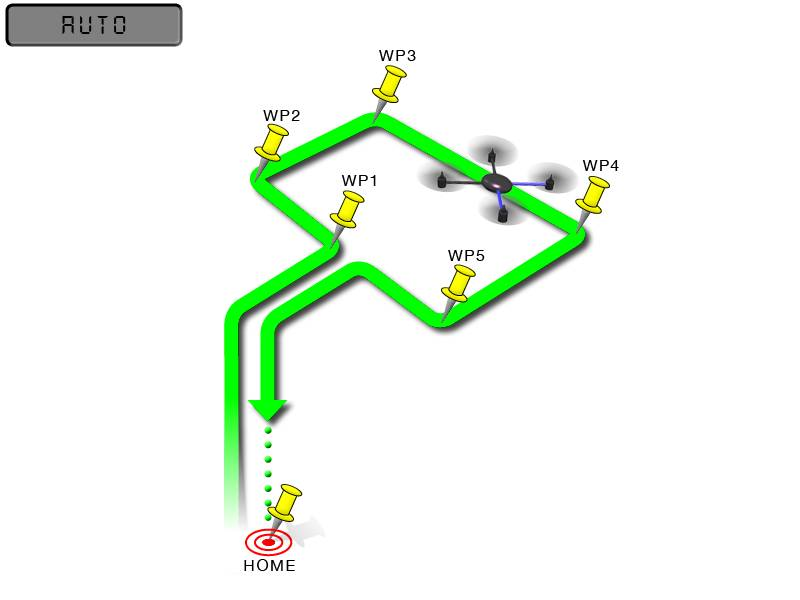
\includegraphics[width=0.7\linewidth]{auto}
	\centering
	\caption{\label{fig: auto}\textit{Overview of Auto Mode}}
\end{figure}
AUTO mode incorporates the altitude control from AltHold mode and position control from Loiter mode and should not be attempted before these modes are flying well as we mentioned above. All the same requirements apply including ensuring that vibration levels and compass interference levels are acceptable and that the GPS is functioning well including returning an HDOP of under 2.0. Figure ~\ref{fig: auto} aptly describes the Auto Mode execution.



\subsubsection{Controls and How it would be executed?}
AUTO should be set-up as one of the Flight Modes on the flight mode switch.

If starting the mission while the copter is on the ground wet should ensure the throttle is down, then we would switch to the Auto flight mode, then raise the throttle. The moment that the throttle is raised above zero, the copter will begin the mission.

If starting the mission from the air the mission will begin from the first command the moment that the flight mode switch is moved to Auto. If the first command in the mission is a take-off command but the vehicle is already above the take-off command’s altitude the take-off command will be considered completed and the vehicle will move onto the next waypoint.

At any time we can retake control (which was needed in our case many times due to poor GPS Connectivity) from the autopilot by returning the flight mode switch to another flight mode such as Stabilize or Loiter. If the pilot then switches to AUTO again, the mission will restart from the first command.

During the mission the our roll, pitch and throttle inputs are ignored but the yaw can be overridden with the yaw stick. This allows us to, for example aim the nose of the copter (which might have a hard mounted camera on it) as the copter flies the mission. The autopilot will attempt to retake yaw control as the vehicle passes the next waypoint. The overall Mission Flight Plan for the above explained Auto-Grid is shown in Fig.~\ref{fig: mp_auto_mission_grid}.

\subsubsection{Ending a Mission}

Missions should normally have an RTL as their final command to ensure the copter will return after the mission completes. Alternatively the final command could be a LAND with a different location. Without a final RTL or LAND command the copter will simply stop at the final waypoint and we will need to retake control with the transmitter.

We should remember that when using RTL, the copter will return to the “home” position which is the location where the copter was armed.

As the copter touches down at the end of the mission we should move the throttle to zero at which point the autopilot will disarm the motors if it also believes that it has landed.



There are detailed reasons why we utilized the above mentioned flight modes in our testing. 



 
\section{Conclusion}

We conducted some tests using the theory and practical approach mentioned earlier in this section. So we can conclude that using the apporach mentioned in this chapter which documented our way of planning a flight in the agricultural/farming area.

Following the approaches mentioned, we are trying to bridge the gap of open-source market with common people. We want to make the data available of crops from the agricultural field from flight data to the researcher's community so that all sorts of testing can be done on a large scale. Hence, we are planning to open source our image dataset we would be taking from an actual agricultural field following a mission as described in Fig.~\ref{fig: mp_auto_mission_grid}.



